\documentclass[compress]{beamer}
\usepackage[T1]{fontenc}
%\usepackage{newtxtext,newtxmath}
\usepackage{lmodern}% http://ctan.org/pkg/lm
\usepackage{pgfpages}
\usepackage{graphicx}
\usepackage{mathtools}          % used for equations


\mode<presentation>{\usetheme{Darmstadt}}
\usefonttheme{professionalfonts} % using non standard fonts for beamer
\usecolortheme{beaver}
\usecolortheme{rose}
\useoutertheme[footline=empty,subsection=false]{miniframes}
\useinnertheme{default}
\setbeamertemplate{items}[default]
\setbeamertemplate{section in toc}[sections numbered]
\setbeamertemplate{subsection in toc}[sections default]
\beamertemplatenavigationsymbolsempty

\setlength{\unitlength}{\textwidth}  % measure in textwidths


\title[Trajectory optimization]{Energy savings for UAV flight in unsteady gusting conditions \\
through trajectory optimization }
\author{Lou Grimaud} % (optional, for multiple authors)
\institute{Illinois Institute of Technology} % (optional)
\date{July 2014} % (optional)

\logo{
\includegraphics[height=0.3cm]{./Figures/IIT_Logo2.eps}}

\begin{document}
\AtBeginSection[]
{
  \begin{frame}
    \frametitle{Table of Contents}
    \tableofcontents[currentsection,currentsubsection]
  \end{frame}
}


\frame{\titlepage}

\begin{frame}
  \frametitle{Table of Contents}
  \tableofcontents
\end{frame}

\section{Introduction}
\begin{frame}
  \frametitle{Introduction and motivations}

\end{frame}

\section[Trajectory optimization]{The trajectory optimization problem}

\subsection{Dynamic soaring}

\begin{frame}
  \frametitle{Different types of soaring}
  \begin{columns}
    \column{.5\textwidth}
    \begin{figure}[h]
      \centering
      %\includegraphics{<+file+>}
      \caption{something about soaring}
    \end{figure}
    \column{.5\textwidth}
    {\Large Spatial wind gradients}
    \begin{itemize}
      \item Thermal updrafts
      \item Horizontal wind gradients
    \end{itemize}
    {\Large Temporal wind gradients}
    \begin{itemize}
      \item Natural turbulences
      \item Building and natural feature wake
    \end{itemize}
  \end{columns}
\end{frame}

\subsection{Neutral energy loop}

\begin{frame}
  \frametitle{Defining the energy extraction problem}
  \begin{columns}
    \column{.5\textwidth}
    What is an ``optimal trajectory''?
    \begin{itemize}
      \item Maximum energy at the end of the cycle
      \item Maximizing the energy gain at each instant of the cycle
      \item \emph{Minimize the energy input needed for sustainable flight}
    \end{itemize}

    \column{.5\textwidth}
    \begin{block}{The neutral energy loop}
      Finding the minimal wind gust that allows to maintain altitude and speed over a gust. 
    \end{block}
  \end{columns}
\end{frame}

\begin{frame}%[shrink]
  \frametitle{Aircraft model\footnote{\tiny Lissaman P and Patel C. Neutral energy cycles for a vehicle in sinusoidal and turbulent vertical gusts. 45th AIAA meeting,863, 2007}}
  \begin{equation*}
    \begin{array}[c]{c}
      m \ddot{x} = -L' \cdot sin(\gamma) + D' \cdot cos(\gamma) \\
      m \ddot{z} = L' \cdot cos(\gamma) - D' \cdot sin(\gamma) - m \cdot g
    \end{array}
  \end{equation*}
  \begin{columns}
    \column{.4\textwidth}
    \begin{figure}[h]
      \centering
      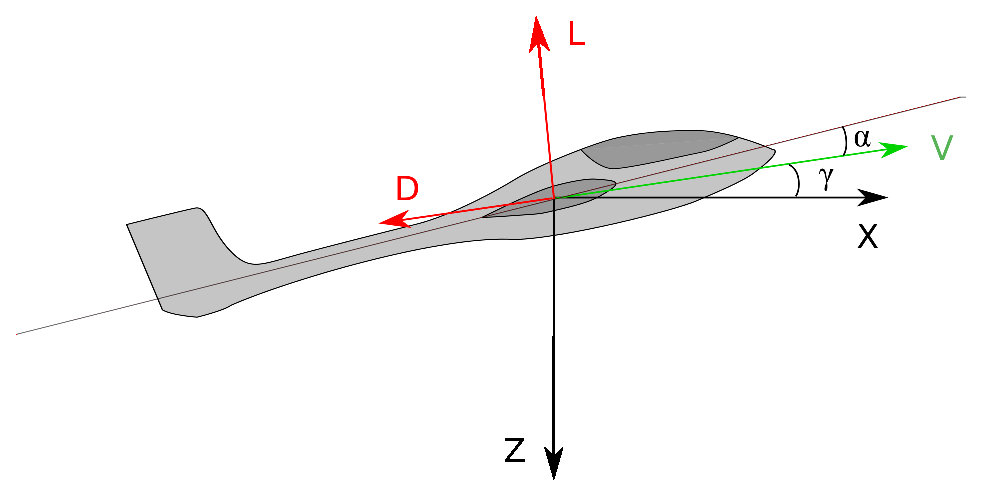
\includegraphics[width=1\textwidth]{./Figures/glider.eps}
      %\caption{Coordinate system used for the optimization}
    \end{figure}
    \column{.7\textwidth}
    Lissaman's non-dimensional variables
    \begin{itemize}
      \item Velocities with $V^{*}$ the optimal glide speed
      \item Time with $T=\frac{V^{*}}{g}$
      \item Lift and drag coefficients $L= \frac{C_l}{C_l^*}$ $D= \frac{C_d}{C_d^*}$
      \item Dynamic pressure $Q = \frac{L'}{MgL} = \frac{ \rho V^{2} C_l^* }{2Mg}$ $Q=(U-U_g)^2+ (W-W_g)^2$
    \end{itemize}
  \end{columns}
  \begin{equation*}
    \begin{array}[c]{c}
      \\
      \frac{dU}{dT}= -LQ \cdot sin(\gamma) + DQ \cdot cos(\gamma) \\
      \frac{dW}{dT}= LQ \cdot cos(\gamma) - DQ \cdot sin(\gamma) - 1
    \end{array}
  \end{equation*}
\end{frame}

\begin{frame}
  \frametitle{Quasi-steady lift and drag model}

  \begin{columns}[t]
    \column{.5\textwidth}
    \begin{itemize}
      \item NACA0009 characteristic
    \end{itemize}
    \column{.5\textwidth}
    \begin{itemize}
      \item Lissaman's quadratic drag
    \end{itemize}
  \end{columns}
  \begin{columns}
    \column{.6\textwidth}
    \begin{figure}[h]
      \centering
      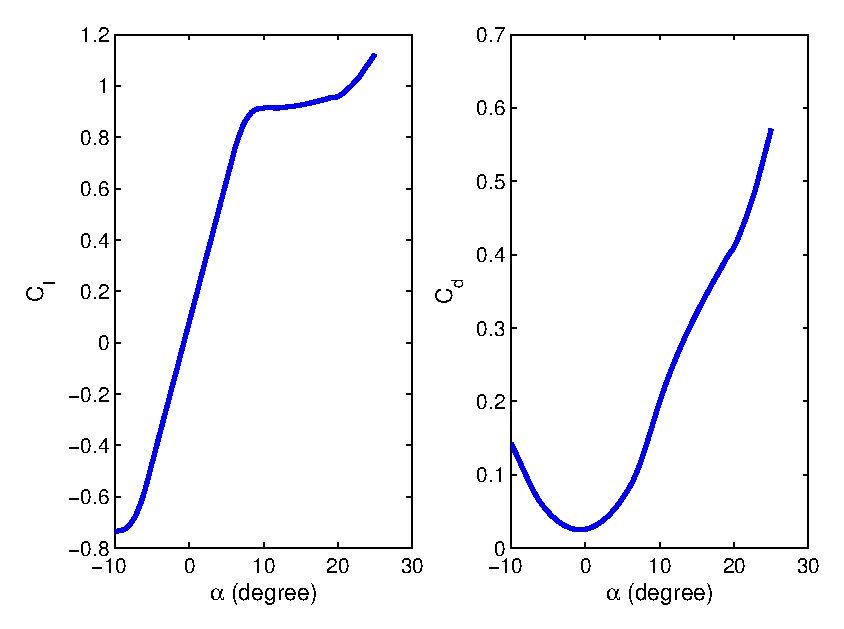
\includegraphics[width=1\textwidth]{./Figures/NACA0009_steady_map_Cl_Cd.eps}
      \caption{Simplified lift and drag for the NACA0009 airfoil}
    \end{figure}
    \column{.4\textwidth}
    \begin{equation*}
      \begin{array}[c]{c}
	D=\frac{1+L^2}{2G^*}\\ \\ \\ \\ 
      \end{array}
    \end{equation*}
  \end{columns}
\end{frame}

\begin{frame}
  \frametitle{Wind profiles}
  We define three different wind profiles:
  \begin{itemize}
    \item Vertical wind gust:
      \begin{equation*}
	\begin{array}[c]{c}
	  W_g = W_a \cdot \sin(2\pi \frac{T}{T_g}) \\
	  U_g = 0 
	\end{array}
      \end{equation*}
    \item Horizontal wind gust:
      \begin{equation*}
	\begin{array}[c]{c}
	  W_g =0 \\ 
	  U_g = W_a \cdot \cos(2\pi \frac{T}{T_g}) 
	\end{array}
      \end{equation*}
    \item Combined wind gust:
      \begin{equation*}
	\begin{array}[c]{c}
	  W_g = W_a \cdot \sin(2\pi \frac{T}{T_g}) \\ 
	  U_g = W_a \cdot \cos(2 \pi \frac{T}{T_g} + \varphi)
	\end{array}
      \end{equation*}
  \end{itemize}
\end{frame}

\begin{frame}
  \frametitle{Optimization algorithm - a minimization problem}
  \begin{itemize}
    \item State vector
      \begin{equation*}
	x= 
	\begin{bmatrix}
	  \cdots \\
	  X_i \\
	  Z_i \\
	  U_i \\
	  W_i \\
	  L_i / \alpha_i \\
	  \cdots \\
	  W_a
	\end{bmatrix}
	\quad i \in [1,N]
      \end{equation*}
    \item Cost function: $W_a$
    \item Constraints: equations of motion, limits on the range of angles of attack allowed, neutral energy loop conditions.
  \end{itemize}
  %state vector and cost function
\end{frame}

\begin{frame}
  \frametitle{Constraints formulation}
  \begin{itemize}
    \item Equations of motion (with Simpson's discreet integral)
      \begin{equation*}
	\begin{array}[c]{cc}
	  y_i= \begin{bmatrix}
	    X_i \\
	    Z_i \\
	    U_i \\
	    W_i 
	  \end{bmatrix} &

	  \dot{y_i} = 
	  \begin{bmatrix}
	    U_i \\
	    W_i \\
	    -L_i Q_i \cdot sin(\gamma_i) + D_i Q_i \cdot cos(\gamma_i) \\
	    L_i Q_i  \cdot cos(\gamma_i ) - D_i Q_i  \cdot sin(\gamma_i ) - 1
	  \end{bmatrix}
	\end{array}
      \end{equation*}

      \begin{equation*}
	0=y_{k+1} - y_k - \frac{1}{6}( \dot{y_k} + 4 \dot{y_m} + \dot{y_{k+1}})\delta t \quad \forall i \in [1,N-1]
      \end{equation*}
  \end{itemize}

  \begin{columns}[t]
    \column{0.5\textwidth}
    \begin{itemize}
      \item Neutral energy loop
	\begin{equation*}
	  \begin{array}[c]{cc}
	    Z_1 = Z_N & L_1 = L_N \\
	    W_1 = W_N & U_1 = U_N
	  \end{array}
	\end{equation*}
	\begin{equation*}
	  \begin{array}[c]{c}
	    W_2 - W_1 = W_N - W_{N-1} \\
	    U_2 - U_1 = U_N - U_{N-1} 
	  \end{array}
	\end{equation*}
    \end{itemize}
    \column{0.5\textwidth}
    \begin{itemize}
      \item Limits in range of $C_l$
	\begin{equation*}
	  \begin{array}[c]{c}
	  L_{\min} \le L_i \le L_{\max} \\
	  \alpha_{\max} \le \alpha_i \le \alpha_{\max}
	  \end{array}
	\end{equation*}
    \end{itemize}
  \end{columns}
\end{frame}

\subsection{Implementation and validation}

\begin{frame}
  \frametitle{Comparison with Lissaman's results - Quadratic model}
Lissaman found a gust amplitude $W_a=0.128$ for this case 
  \begin{columns}
    \column{0.5\textwidth}
    \begin{figure}[ht]
      \begin{center}	
	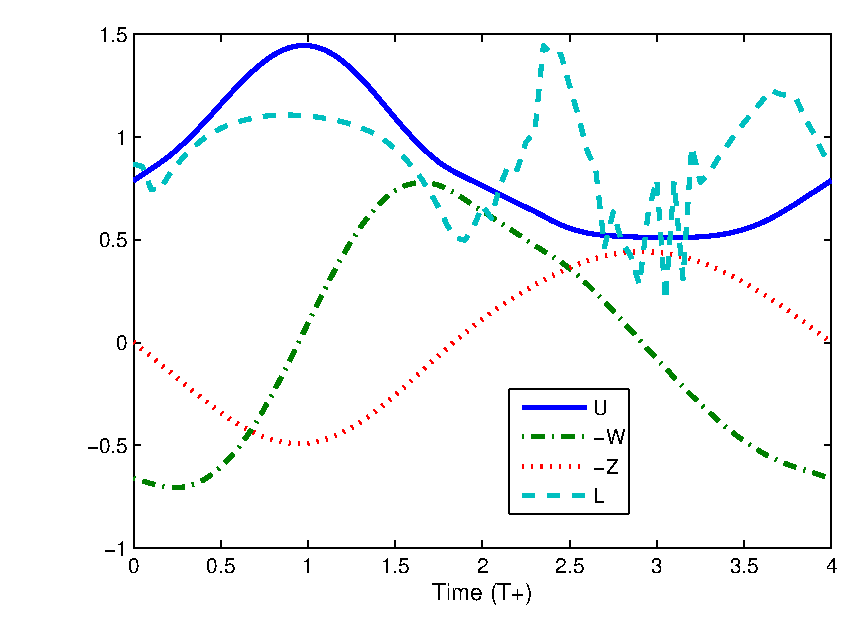
\includegraphics[width=1\textwidth]{./Figures/Windtype=1_Tg=4_Wg=0p129_quad_G=20.eps}
      \end{center}
      \caption{Optimization results for a $4T$ long vertical gust $W_a=0.129$}
    \end{figure}
    \column{0.5\textwidth}
    \begin{figure}[h]
      \centering
      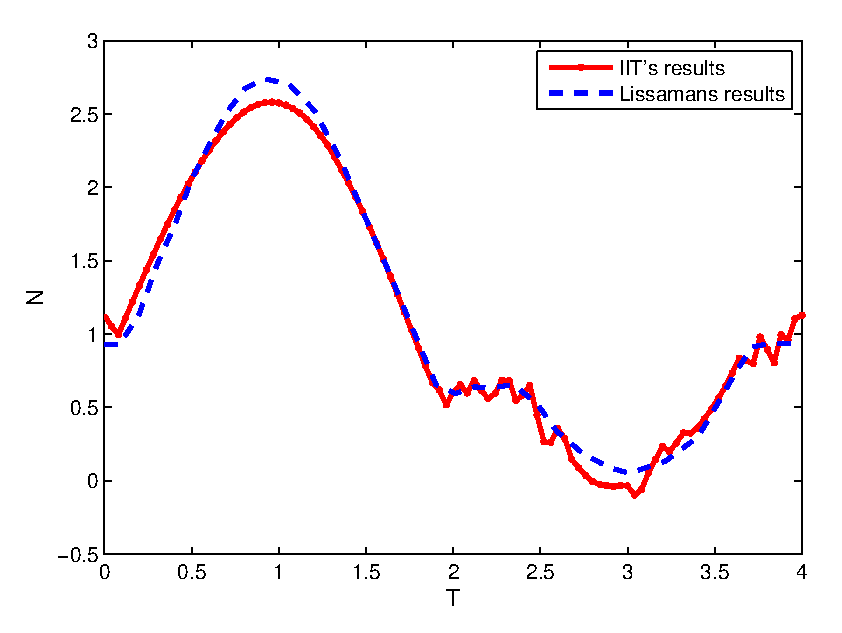
\includegraphics[width=1\textwidth]{./Figures/LIssaman_N_comparison.eps}
      \caption{Comparison with Lissaman's non-dimensional normal force $N$ for a $4T$ long vertical gust}
    \end{figure}
  \end{columns}
  %put the lissaman quadratic thing here
\end{frame}

\begin{frame}
  \frametitle{Quasi-steady lift to drag model - NACA009}
  \begin{columns}
    \column{0.5\textwidth}
    \begin{figure}
      \begin{center}
	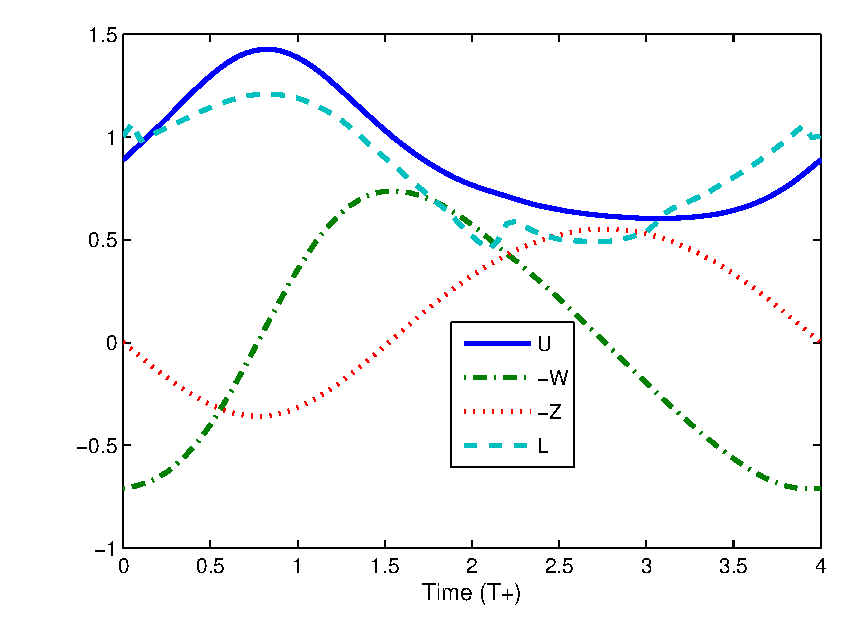
\includegraphics[width=1\textwidth]{./Figures/Windtype=1_Tg=4_Wg=0p205_UAV_alphamax=12.eps}
      \end{center}
      \caption{$4T$ long vertical gust for the NACA0009 airfoil, $W_a=0.205$}
    \end{figure}
    \column{0.5\textwidth}
    \begin{figure}[h]
      \begin{center}
	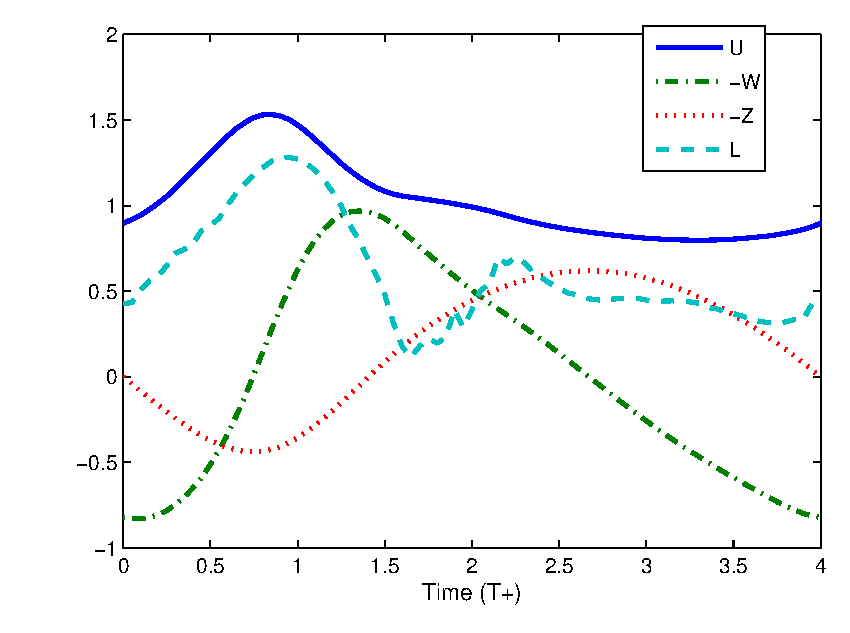
\includegraphics[width=1\textwidth]{./Figures/Windtype=3_Tg=4_Wg=0p387_UAV_alphamax=12.eps}
      \end{center}
      \caption{$4T$ long combined gust for the NACA0009 airfoil, $W_a=0.387$}
    \end{figure}
  \end{columns} % NACA009 curves
\end{frame}

\subsection{Quasi-steady aerodynamic model results}

\begin{frame}
  \frametitle{Tg dependency}
  \begin{columns}
    \column{0.5\textwidth}
    \begin{figure}[h!]
      \begin{center}
	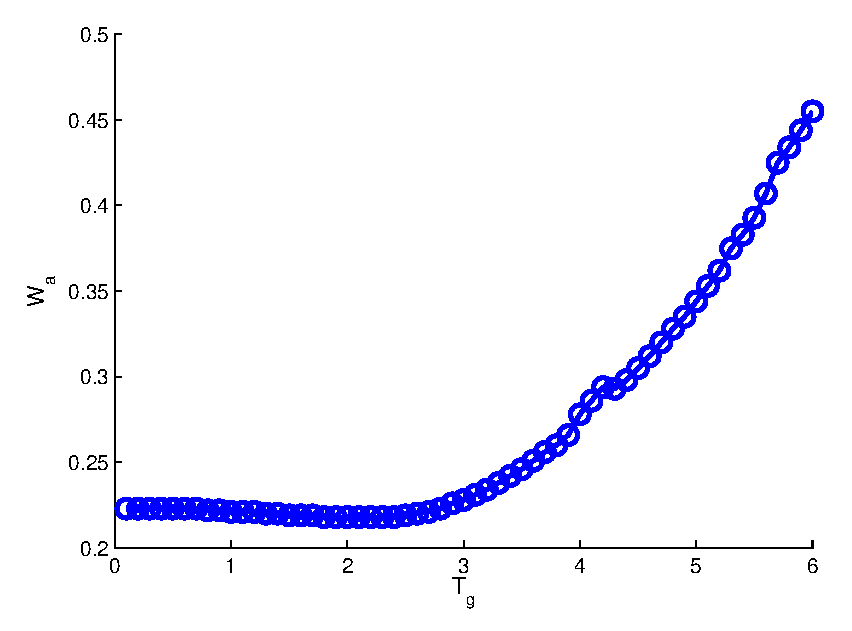
\includegraphics[width=1\textwidth]{./Figures/Wg_vs_TG_windtype=1_alhpamax=12_nodalphalimit.eps}
      \end{center}
      \caption{Influence of gust duration on the minimum gust amplitude for vertical gusts}
      \label{fig:vertical_amplitude_duration}
    \end{figure}
    \column{0.5\textwidth}
    \begin{figure}[h!]
      \begin{center}
	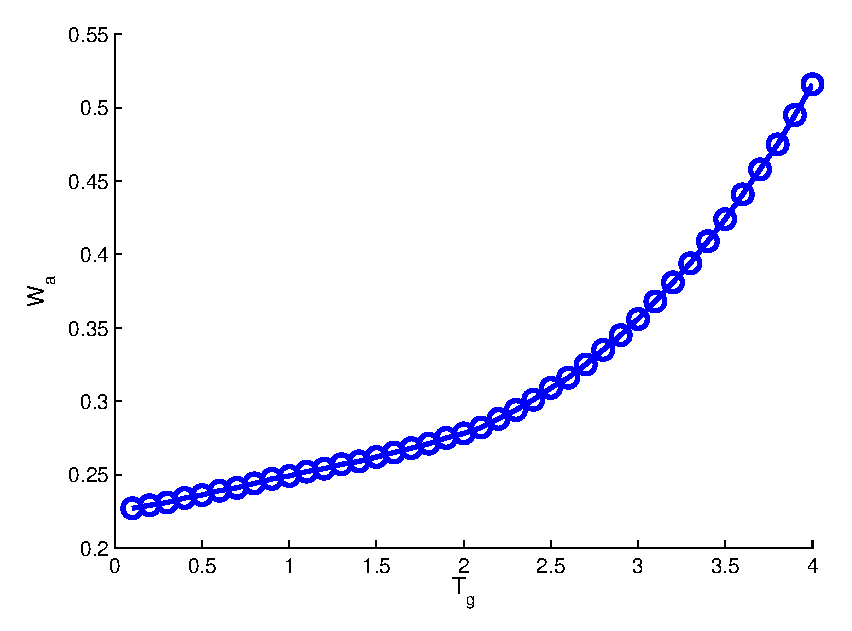
\includegraphics[width=1\textwidth]{./Figures/Wg_vs_TG_windtype=3_alhpamax=12_nodalphalimit.eps}
      \end{center}
      \caption{Influence of gust duration on the minimum gust amplitude for combined gusts}
      \label{fig:combined_amplitude_duration}
    \end{figure}
  \end{columns} % NACA009 curves
\end{frame}

\begin{frame}
  \frametitle{Difference between short and long gusts}
  We can see that there is tipping point around $T_g=2.5$
  \begin{figure}[h]
    \centering
    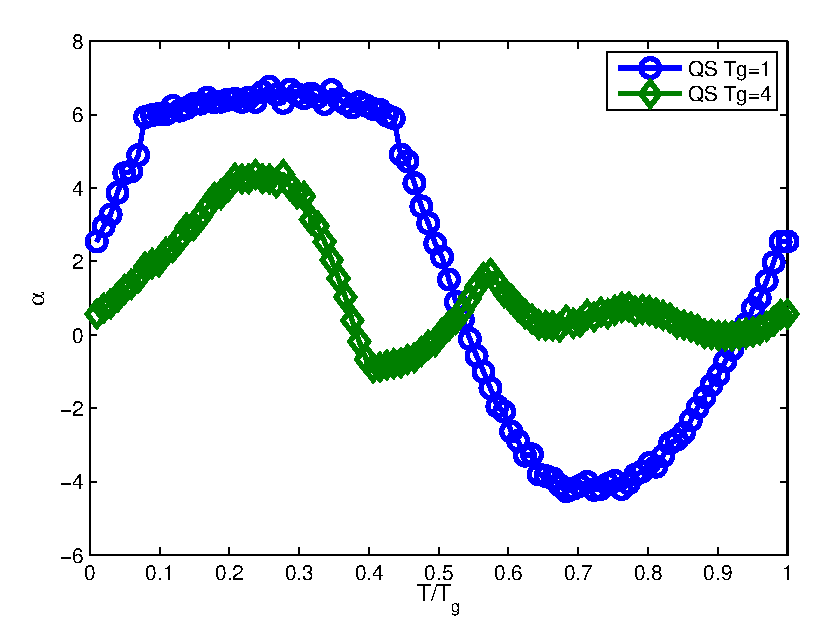
\includegraphics[width=0.7\textwidth]{./Figures/alpha_vs_Tg_QS_short_vs_long_wt3.eps}
    \caption{Difference between short and long gust angle of attack profile for combined gusts}
    \label{fig:short_vs_long_qs_wt=3}
  \end{figure}
\end{frame}

\begin{frame}
  \frametitle{Angle of attack limitation}
  \begin{columns}
    \column{0.5\textwidth}
    \begin{figure}[h]
      \centering
      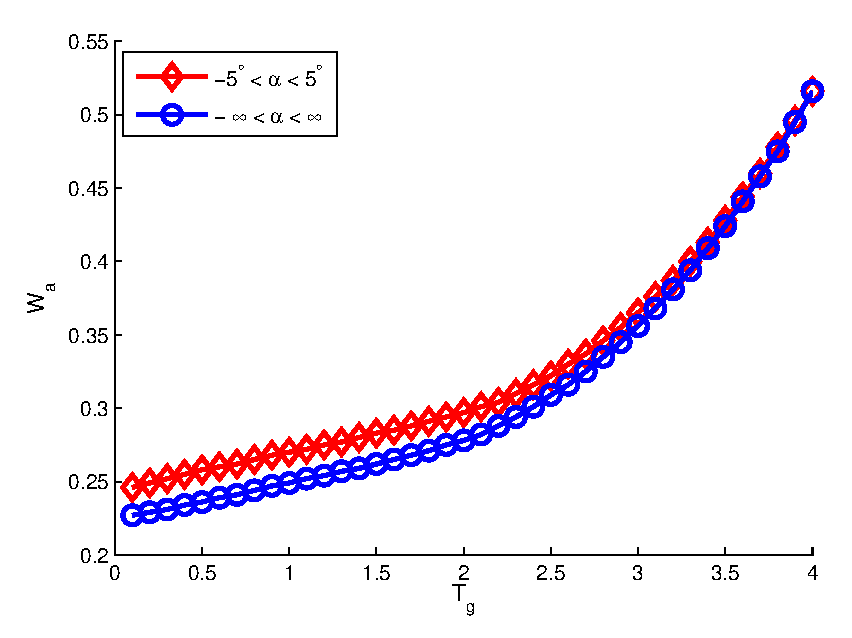
\includegraphics[width=1\textwidth]{./Figures/allowed_alpha_wg_tg_wt=3.eps}
      \caption{Difference in performance for combined wind gusts if no high angle of attack are allowed}
      \label{fig:allowed_alpha_Wt_vs_tg_wt=3}
    \end{figure}

    \column{0.5\textwidth}
    \begin{figure}[h]
      \centering
      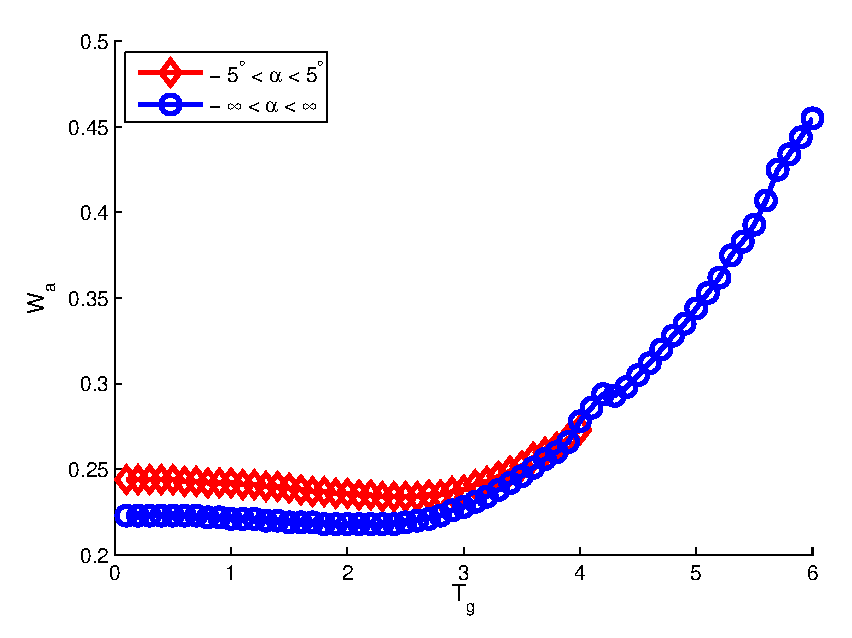
\includegraphics[width=1\textwidth]{./Figures/allowed_alpha_wg_tg_wt=1.eps}
      \caption{Difference in performance for vertical wind gusts if no high angle of attack are allowed}
      \label{fig:allowed_alpha_Wt_vs_tg_wt=1}
    \end{figure}
  \end{columns}
\end{frame}

\begin{frame}
  \frametitle{Phase influence}
  \begin{figure}[ht]
    \begin{center}
      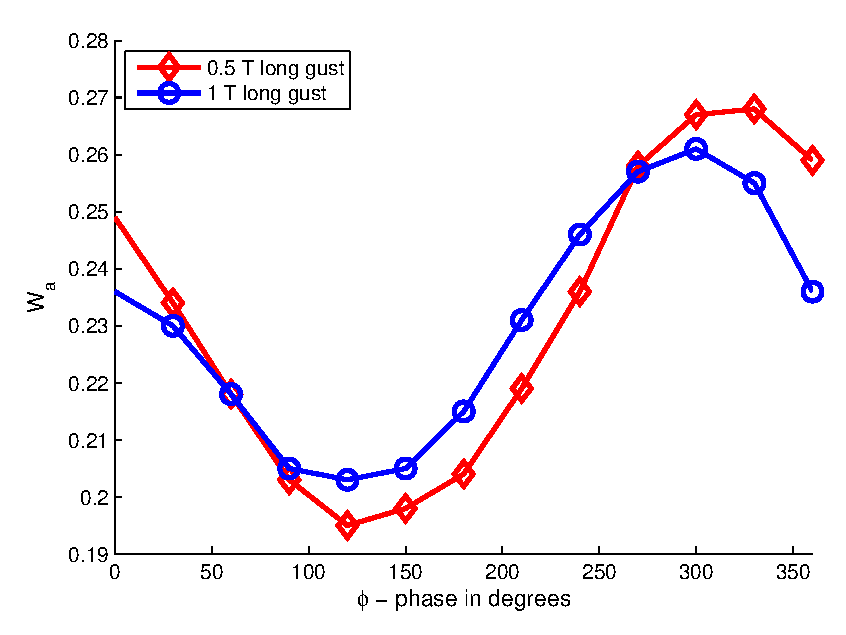
\includegraphics[width=0.7\textwidth]{./Figures/combined_gust_amplitude_vs_phase_LUT.eps}
    \end{center}
    \caption{Influence of the phase between the components of the combined gust}
    \label{fig:combined_amplitude_phase}
  \end{figure}
\end{frame}


\section[GK model]{The unsteady pitching aerodynamic model}

\subsection{Experimental setup}

\begin{frame}[shrink]
  \frametitle{Pitching mechanism and experimental conditions}
  \begin{columns}
    \column{0.6\textwidth}
    \begin{figure}[h]
      \begin{center}
	\includegraphics[width=1.0\textwidth]{./Figures/airfoil_model.eps}
      \end{center}
      \caption{Airfoil model inside the wind tunnel}
    \end{figure}
    \column{0.5\textwidth}
    Experimental conditions
    \begin{itemize}
      \item Free stream velocity: 3 m/s
      \item Airfoil: NACA0009
      \item Reynolds number ~50000
    \end{itemize}
    Controller and data acquisition
    \begin{itemize}
      \item Angle of attack controlled by simulink\textsuperscript{\textregistered} and two servomotors 
      \item Servos position measured by two linear potentiometers
      \item Piezoelectric force balance (NANO17) to measure the forces on the airfoil
    \end{itemize}
  \end{columns}
\end{frame}

\subsection{The Goman and Khrabrov model}

\begin{frame}
  \frametitle{The GK model concept}
  The Goman and Khrabrov model\footnote{Goman M and Khrabrov A. \emph{Journal of Aircraft}, 31(5):1109–1115,1994.} - a non-linear state space model
  \begin{equation*}
    \begin{array}[c]{c}
      C_l= f(\alpha,x) \\
      C_d= g(\alpha,x) \\
      \tau_1 \frac{dx}{dt} +x = x_0(\alpha - \tau_2 \dot{\alpha}) 
    \end{array}
  \end{equation*}

  \begin{columns}[t] 
    \column{0.38\textwidth}
    \begin{itemize}
      \item   \textbf{Lift and drag model}
    \end{itemize}
    \column{0.38\textwidth}
    \begin{itemize}
      \item    \textbf{Non-linear state map}
    \end{itemize}
    \column{0.38\textwidth}
    \begin{itemize}
      \item \textbf{Time constants $\tau_1$ and $\tau_2$} 
    \end{itemize}
  \end{columns}

  \begin{columns}
    \column{0.4\textwidth}
    \resizebox{\textwidth}{!}{%
      $
      \begin{array}[c]{c}
	\\
	C_l=2 \pi \alpha (0.6 x + 0.4) + C_{l0} \\
	C_d= \frac{ \left( \left( 2 - x \right)C_l \right)^2 }{G_{\max}} + C_{d0}
      \end{array}
      $%
    }
    \column{0.4\textwidth}
    \begin{figure}[h]
      \begin{center}
	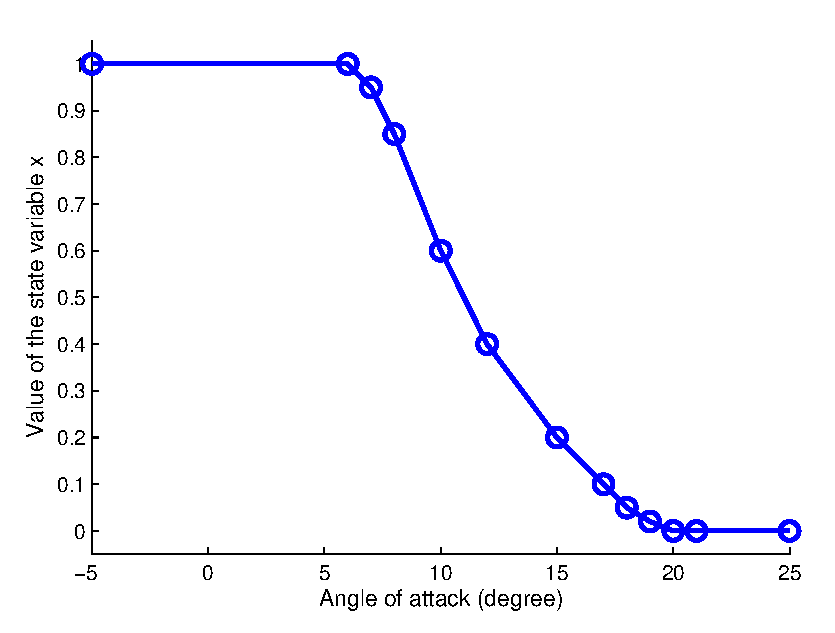
\includegraphics[width=0.9\textwidth]{./Figures/x_0_vs_alpha.eps}
      \end{center}
    \end{figure}
    \column{0.4\textwidth}
    \begin{figure}[h]
      \begin{center}
	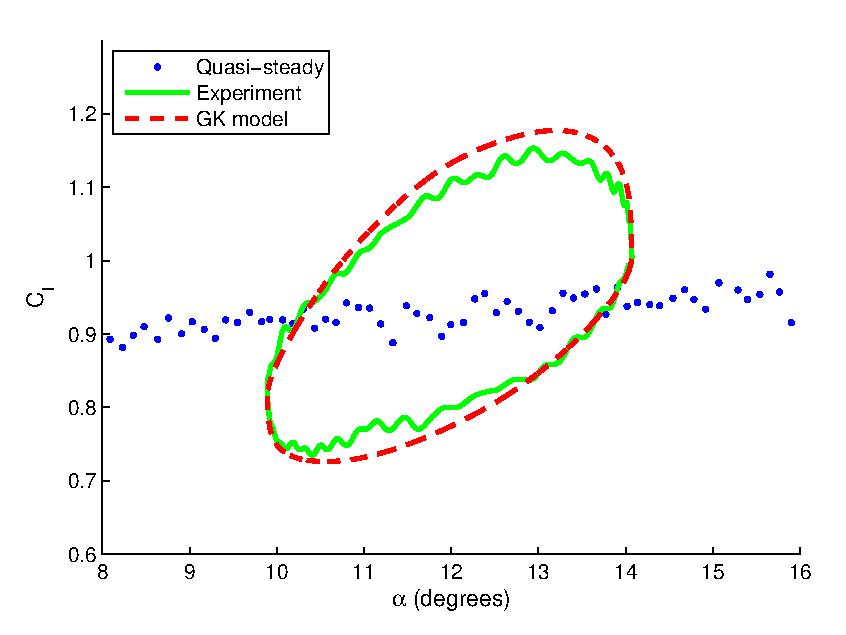
\includegraphics[width=0.9\textwidth]{./Figures/Cl_u=3_meanaoa=12_amp=2_freq=0p5.eps}
      \end{center}
    \end{figure}

  \end{columns}
\end{frame}

\subsection{Determination and validation of the model}

\begin{frame}
  \frametitle{Quasi-steady map and state variable}
  \begin{equation*}
      \begin{array}[c]{c}
	C_l=2 \pi \alpha (0.6 x + 0.4) + C_{l0} \\
	C_d= \frac{ \left( \left( 2 - x \right)C_l \right)^2 }{G_{\max}} + C_{d0}
      \end{array}
  \end{equation*}
  \begin{columns}
    \column{0.5\textwidth}
    \begin{figure}[h]
      \begin{center}
	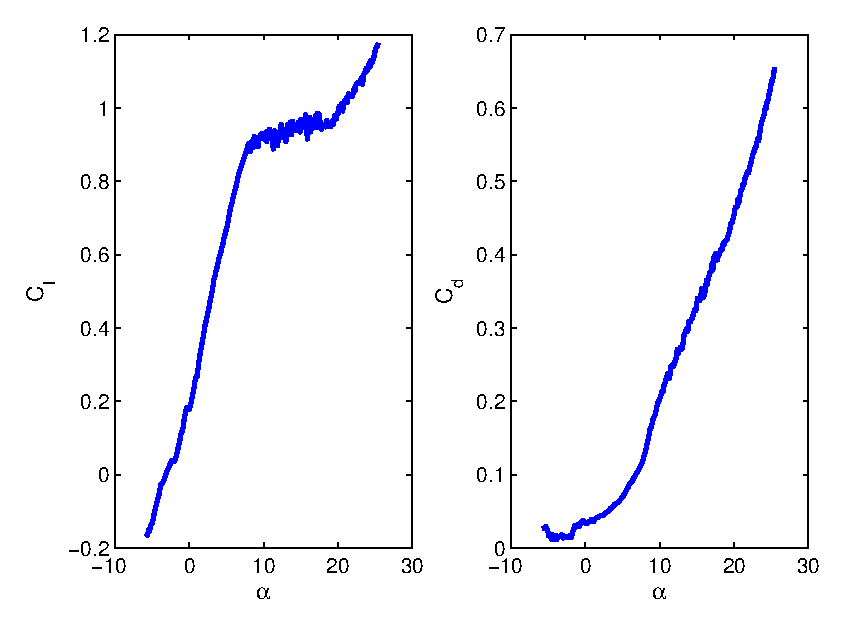
\includegraphics[width=1\textwidth]{./Figures/Cd_and_Cl_NACA0009.eps}
      \end{center}
      \caption{Lift and drag coefficient in the quasi-steady case}
    \end{figure}
    \column{0.5\textwidth}
    \begin{figure}[ht]
      \begin{center}
	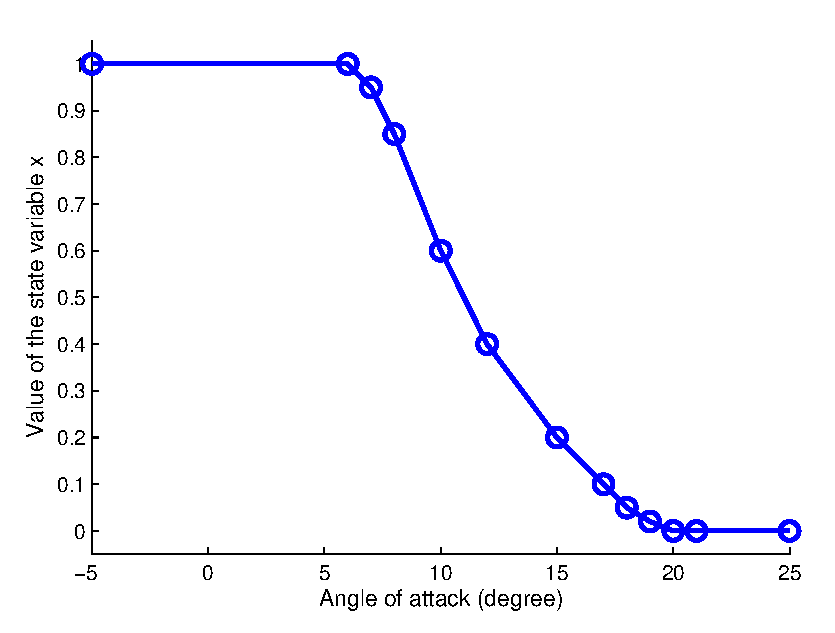
\includegraphics[width=1\textwidth]{./Figures/x_0_vs_alpha.eps}
      \end{center}
      \caption{Quasi-steady profile for the state variable $x$}
    \end{figure}
  \end{columns}
\end{frame}

\begin{frame}
  \frametitle{Time constant determination}
  Periodic sinusoidal pitching at different frequencies $k=\pi \frac{c f}{u}$

  \begin{figure}[h]
    \begin{center}
      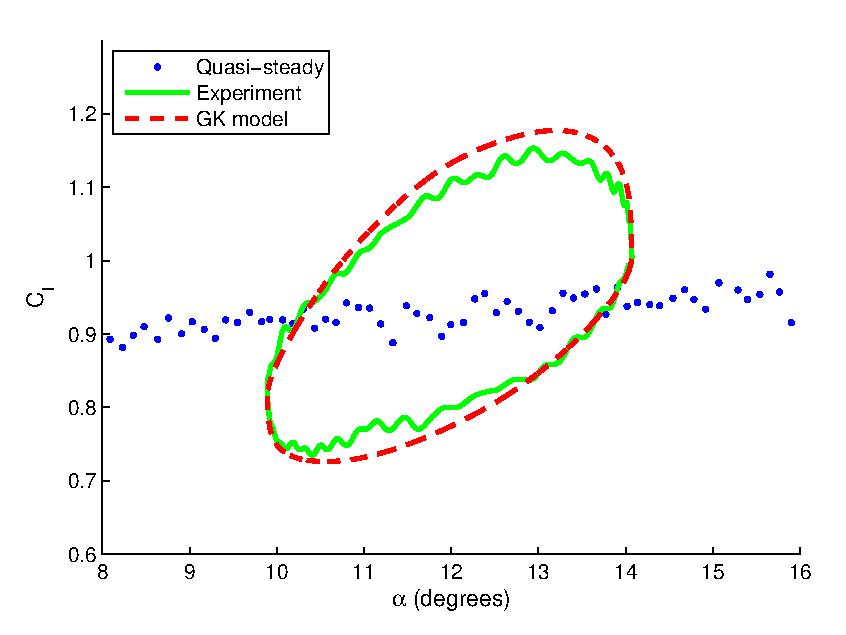
\includegraphics[width=0.65\textwidth]{./Figures/Cl_u=3_meanaoa=12_amp=2_freq=0p5.eps}
    \end{center}
    \caption{Comparison of experimental lift coefficient and model prediction after tunning of the time constant at $k=0.128$}

    We find $\bold{\tau_1=3.1t^+}$ and $\bold{\tau_2=4.29t^+}$ (with $t^+=\frac{c}{u}$)
  \end{figure}
\end{frame}

\begin{frame}
  \frametitle{Comparison with periodic measurements - Lift }

  \begin{figure}[h]
    \begin{center}
      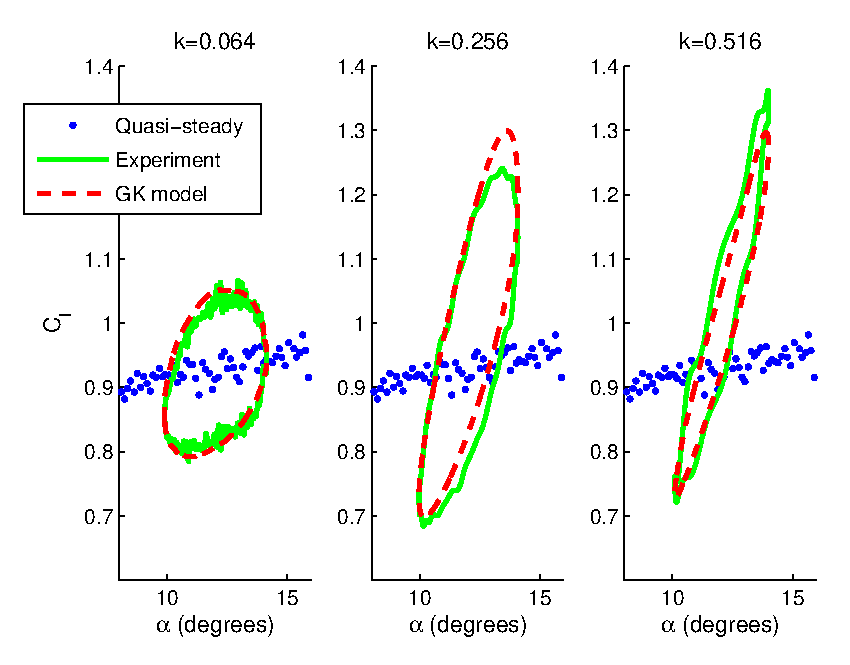
\includegraphics[width=0.75\textwidth]{./Figures/Pitching_allcases_GK_CL_12_amp_2.eps}
    \end{center}
    \caption{Lift measurement and prediction during sinusoidal pitching around 12 degree} 
  \end{figure}
\end{frame}

\begin{frame}
  \frametitle{Comparison with periodic measurements - Drag}

  \begin{figure}[h]
    \begin{center}
      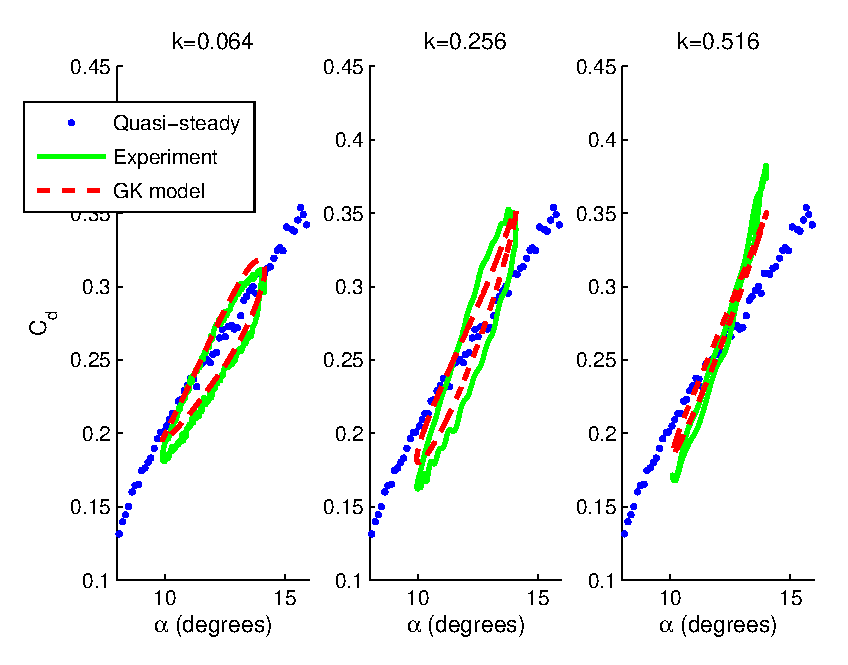
\includegraphics[width=0.75\textwidth]{./Figures/Pitching_allcases_GK_CD_12_amp_2.eps}
    \end{center}
    \caption{drag measurement and prediction during sinusoidal pitching around 12 degree} 
  \end{figure}
\end{frame}

\begin{frame}
  \frametitle{Pseudo-random case - Lift}
  \begin{figure}[h]
    \begin{center}
      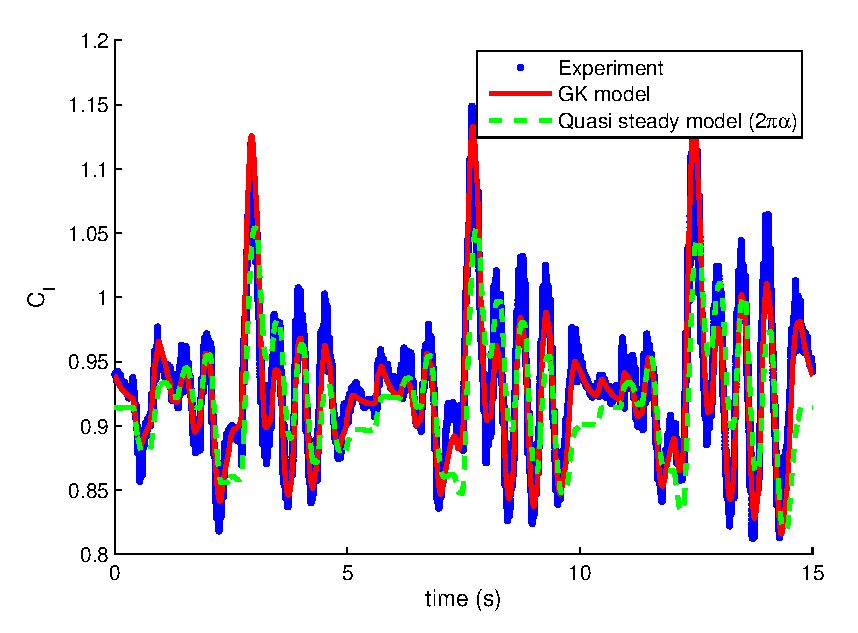
\includegraphics[width=0.8\textwidth]{./Figures/Cl_u=3_meanaoa=12(15seconds)_amp=2_freq=2p0.eps}
    \end{center}
    \caption{Unsteady effects of random pitching on the lift}
  \end{figure}
\end{frame}

\begin{frame}
  \frametitle{Pseudo-random case - Drag}
  \begin{figure}[h]
    \begin{center}
      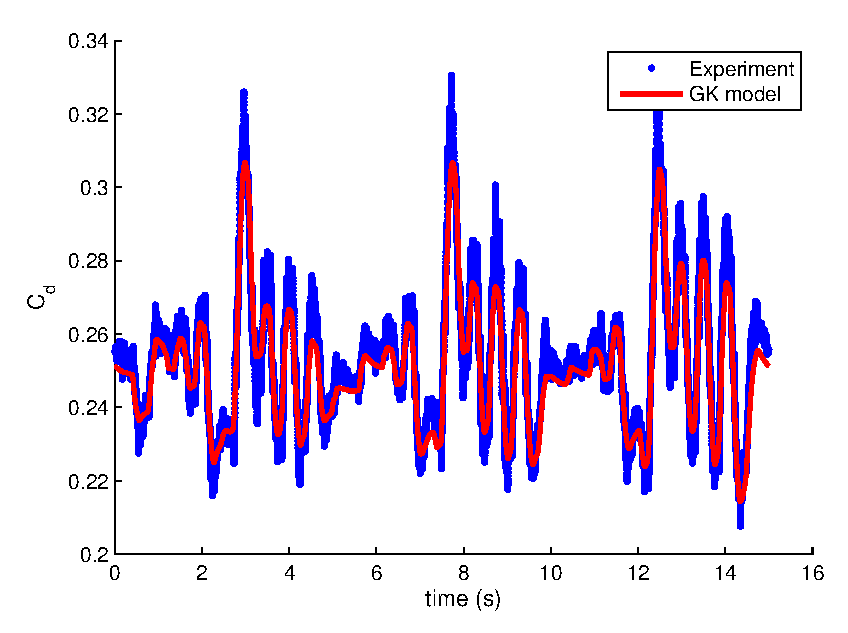
\includegraphics[width=0.8\textwidth]{./Figures/Cd_u=3_meanaoa=12(15seconds)_amp=2_freq=2p0.eps}
    \end{center}
    \caption{Unsteady effects of random pitching on the drag}
  \end{figure}
\end{frame}

\section[Unsteady optimization]{Unsteady trajectory optimization}

\subsection{Time constant equivalence}

\begin{frame}
  \frametitle{Froude number equivalence}
  \begin{columns}
    \column{0.4\textwidth}
    Gliding vehicle time scale
    \begin{equation*}
      T=\frac{g}{V^*}
    \end{equation*}

    Airfoil time scale
    \begin{equation*}
      t^+=\frac{c}{u}
    \end{equation*}

    For a vehicle flying at $V^*$
    \begin{equation*}
      Fr=\frac{T}{t+}=\frac{{V^*}^2}{g \cdot c}
      \label{eqn:T_t+_ratio}
    \end{equation*}

    \column{0.7\textwidth}
    \begin{figure}[h]
      \begin{center}
	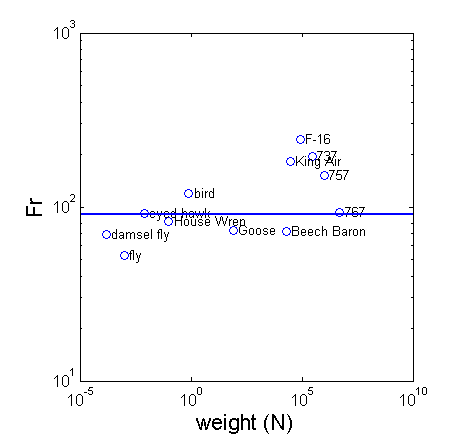
\includegraphics[width=0.8\textwidth]{./Figures/froude.png}
      \end{center}
      \caption{T to t+ ratio for various flying objects}
    \end{figure}
  \end{columns}
\end{frame}
\subsection{Gust duration dependency}

\begin{frame}
  \frametitle{Difference with the quasi-steady model optimization}

  \begin{figure}[h]
    \centering
    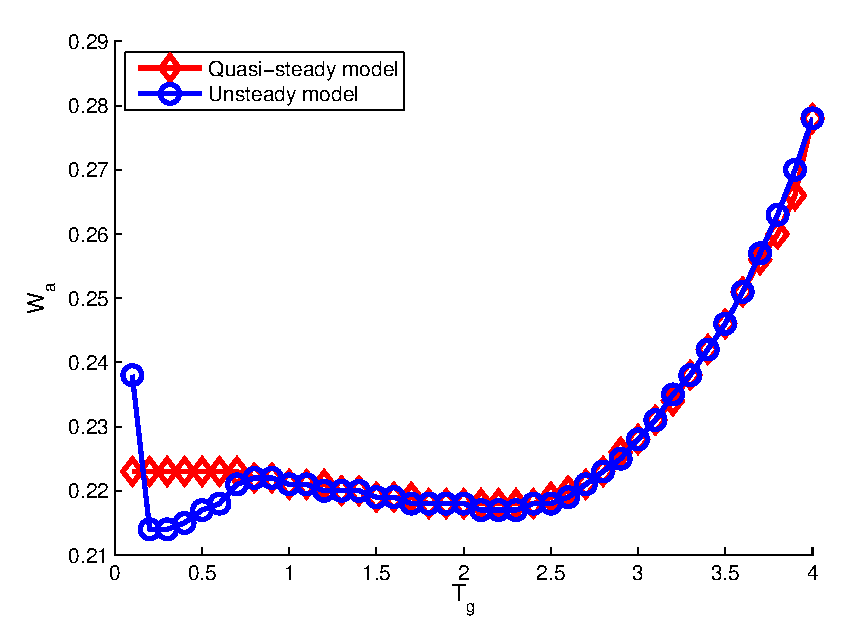
\includegraphics[width=0.8\textwidth]{./Figures/LUT_vs_GK_Wg_vs_TG_windtype=1_alhpamax=12_nodalphalimit.eps}
    \caption{Performance difference between quasi-steady and unsteady model for vertical gusts}
  \end{figure}
\end{frame}


\begin{frame}
  \frametitle{Difference with the quasi-steady model optimization}

  \begin{figure}[h]
    \centering
    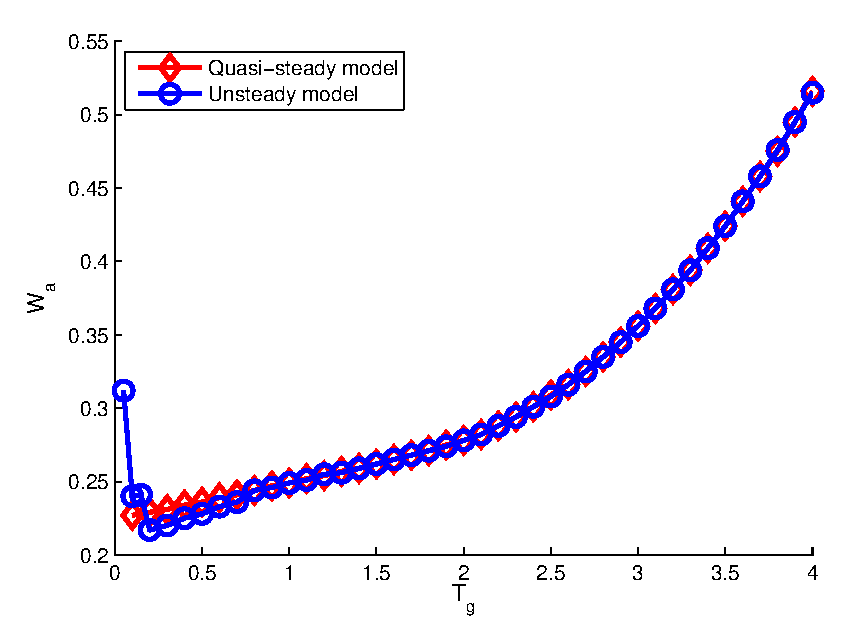
\includegraphics[width=0.8\textwidth]{./Figures/LUT_vs_GK_Wg_vs_TG_windtype=3_alhpamax=12_nodalphalimit.eps}
    \caption{Performance difference between quasi-steady and unsteady model for combined gusts}
  \end{figure}
\end{frame}


\begin{frame}
  \frametitle{A closer look at $T_g \in [0.2,0.5]$ ($k \in [0.05,0.175]$)}
  \begin{figure}[h]
    \centering
    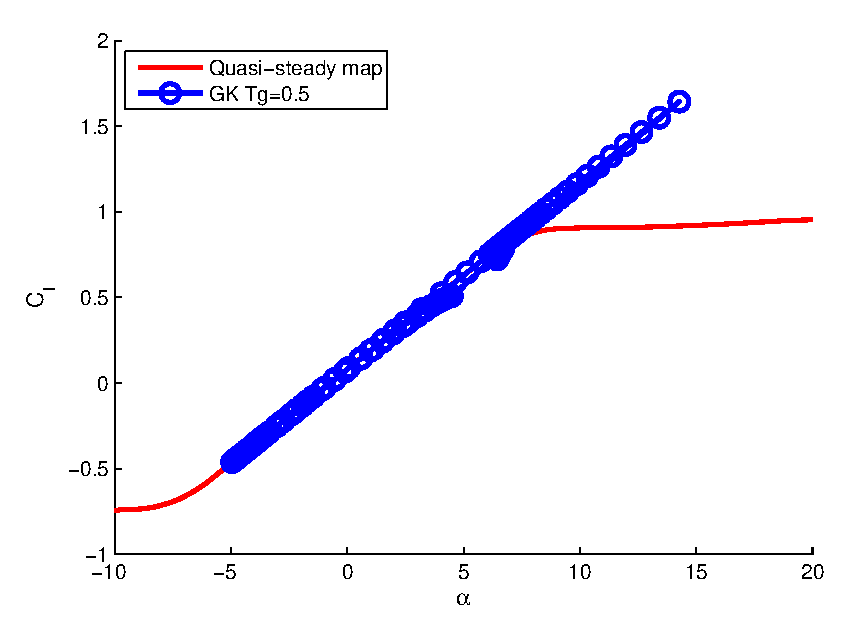
\includegraphics[width=0.8\textwidth]{./Figures/Cl_vs_alpha_wt=1_tg=0p5_alphamax=20.eps}
    \caption{Lift coefficient versus angle of attack for 0.5T long vertical wind gusts with the unsteady model}
  \end{figure}
\end{frame}

\begin{frame}
  \frametitle{A closer look at good performing short gusts}
  \begin{figure}[h]
    \centering
    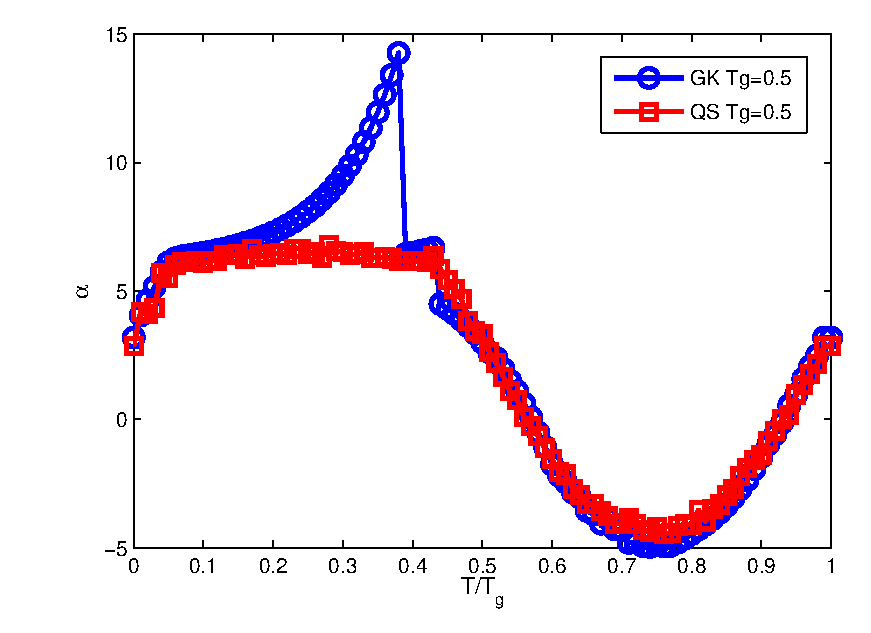
\includegraphics[width=0.8\textwidth]{./Figures/alpha_vs_Tg_wt1.eps}
    \caption{Angle of attack for short vertical gusts with the quasi-steady (QS) and unsteady (GK) model}
  \end{figure}
\end{frame}


\begin{frame}
  \frametitle{Difference around $T_g \le0.2$ ($k \ge 0.175$)}
  \begin{figure}[h]
    \centering
    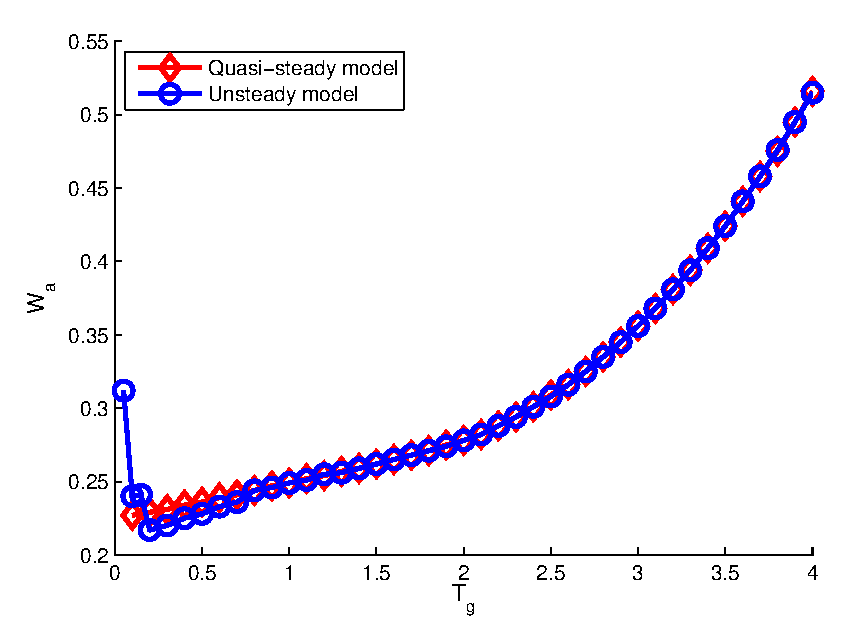
\includegraphics[width=0.8\textwidth]{./Figures/LUT_vs_GK_Wg_vs_TG_windtype=3_alhpamax=12_nodalphalimit.eps}
    \caption{Performance difference between quasi-steady and unsteady model for combined gusts}
  \end{figure}
\end{frame}

\begin{frame}
  \frametitle{Difference around $T_g \le0.2$}

  \begin{figure}[h]
    \centering
    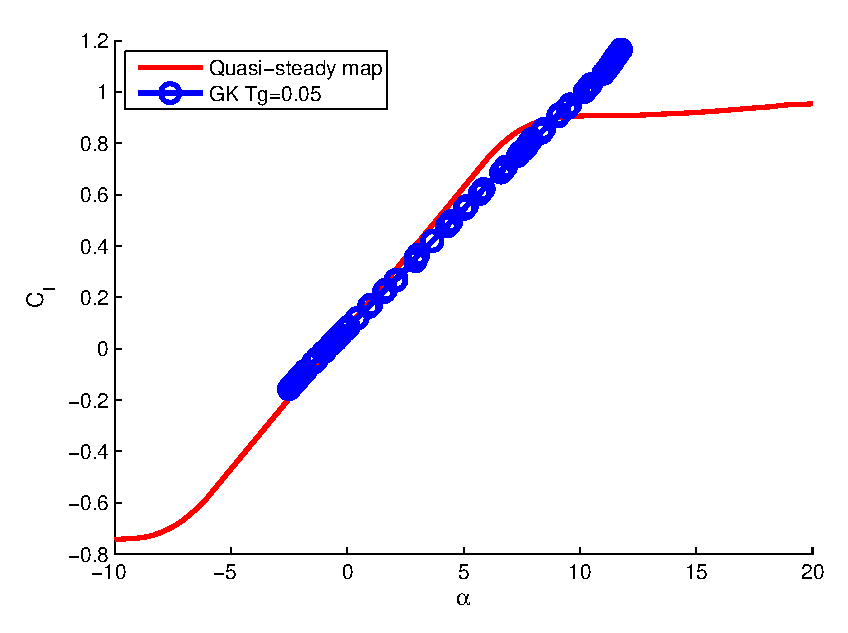
\includegraphics[width=0.9\textwidth]{./Figures/Cl_vs_alpha_Windtype=3_Tg=0p05_GK_alphamax=12.eps}
    \caption{Lift coefficient versus angle of attack for a 0.05T long combined gust}
  \end{figure}
\end{frame}

\subsection{Phase results}

\begin{frame}
  \begin{figure}[h]
    \centering
    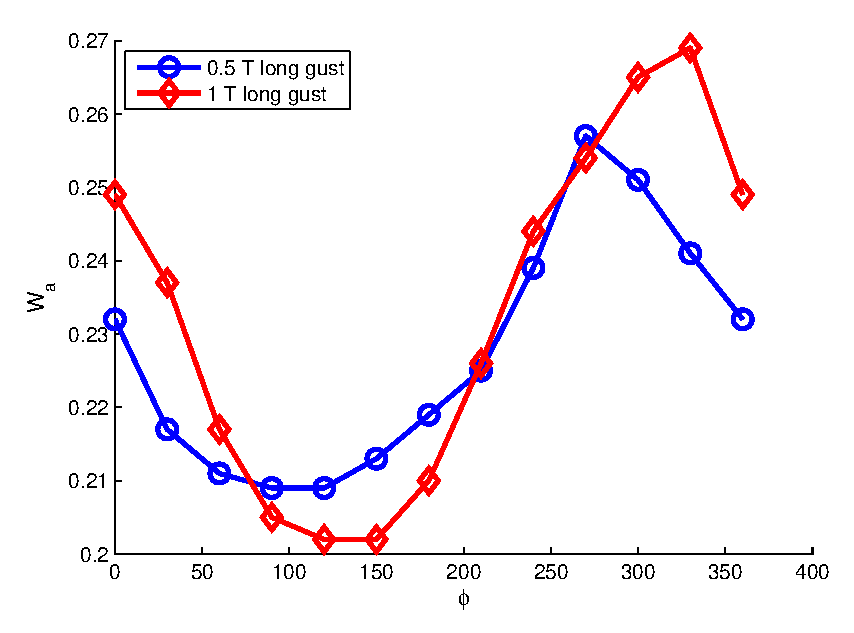
\includegraphics[width=0.8\textwidth]{./Figures/combined_gust_amplitude_vs_phase_GK.eps}
    \caption{Influence of the phase between the components of the combined gust in the unsteady model case}
  \end{figure}
\end{frame}

\begin{frame}

  \begin{figure}[h]
    \centering
    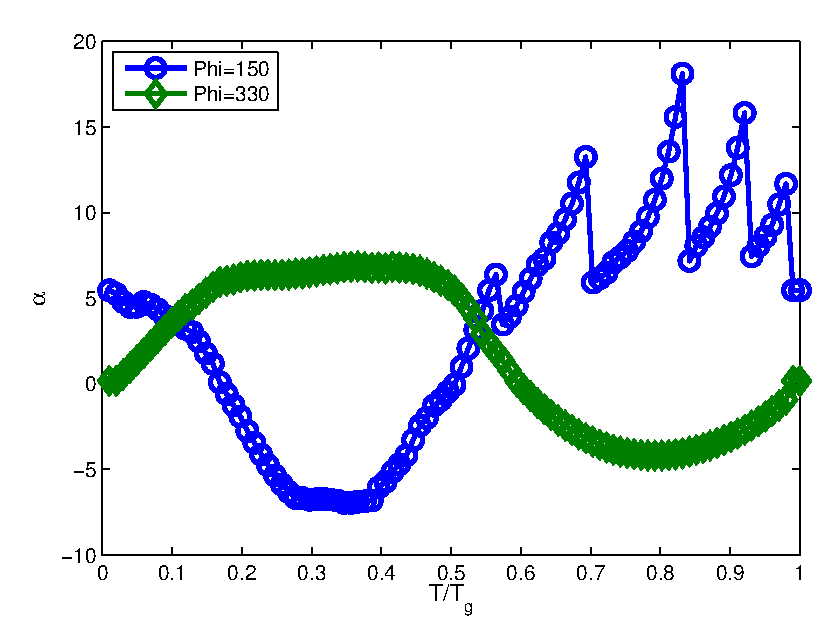
\includegraphics[width=0.9\textwidth]{./Figures/alpha_vs_Tg_GK_phi_Tg=1.eps}
    \caption{Angle of attack profile for different phase angle when $T_g=1$}
  \end{figure}
\end{frame}

\section{Conclusion}
\begin{frame}
  \textbf{GK model prediction:}
  \begin{itemize}
    \item Accurate prediction of lift and \emph{drag} for arbitrary pitch motion
    \item The drag coefficient shares the same state variable as the lift 
    \item The model is fast enough to be used for optimization algorithms
  \end{itemize}
  \textbf{Trajectory optimization}
  \begin{itemize}
    \item Neutral energy flight is possible through combinations of vertical and horizontal gusts
    \item Vehicle and airfoil time scale are related through the Froude number
    \item Unsteady aerodynamic effects are seen for gusts shorter than $0.7T$
    \item The unsteady effects are beneficial for $T_g \in [0.2,0.7]$ as they let the airfoil achieve higher $C_l$ values
    \item The unsteady effects are detrimental for $T_g$ smaller than $0.2$, where the ``angle of attack lag'' becomes significant
  \end{itemize}
\end{frame}

\begin{frame}
  \frametitle{Possible improvements}
  \textbf{GK model prediction:}
  \begin{itemize}
    \item Extending the GK model to a plunging and surging flow
    \item Devise a more rigorous way to obtain the time constants
    \item Implement a model for the moment coefficient
    \item Link the state variable and the flow configuration
  \end{itemize}
  \textbf{Trajectory optimization}
  \begin{itemize}
    \item Further investigations should be performed for very short gusts
    \item The effects of surging and plunging are not considered
    \item Introduce a 3rd degree of freedom to account for the moment of inertia
  \end{itemize}
\end{frame}
\end{document}
